\textit{Alvarenga p619 - Ejercicio 10 y 11}

Considere un rayo luminoso que incide sobre una superficie reflejante en la forma indicada en la figura de este problema.

\begin{enumerate}
    \item Trace en dicha figura la normal a la superficie en el punto de incidencia.
    \item ¿Cuál es el valor del ángulo de incidencia?
    \item ¿Cuál será el valor del ángulo de reflexión?
    \item Trace entonces en la figura la dirección del rayo reflejado.
\end{enumerate}

Responda las mismas preguntas, pero considerando el haz incidente a 40° del haz incidente.

\begin{figure}[h!]
    \centering
    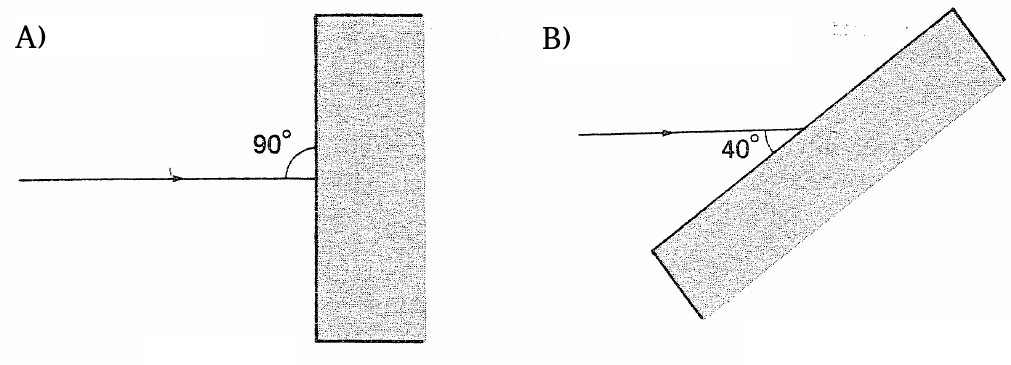
\includegraphics[width=0.6\linewidth]{enunciados/figuras/Prob10_alvarenga619.png}
    \caption{A) Superficie reflejante perpendicular al haz incidente. B) Superficie reflejante a 40° del haz incidente.}
\end{figure}
